% \documentclass[twocolumn, 10pt]{article}
\documentclass[twocolumn,9pt]{extarticle}

\usepackage{geometry}
\geometry{
	a4paper,
	total={6.85in, 9.92in},
	left=0.71in,
	top=0.63in,
}

% \usepackage{hyperref}
% \usepackage[hidelinks]{hyperref}
% \hypersetup{
%     colorlinks = true,   % Use colored text instead of boxes
%     linkcolor = gray,    % Color for internal links (e.g., \ref, \cite)
%     citecolor = blue,    % Color for citations
%     filecolor = magenta, % Color for file links
%     urlcolor = gray      % Color for URLs
% }

\usepackage{graphicx}
\usepackage{xcolor}
\usepackage{caption}

\usepackage{enumitem}
% \setlist{nosep}
\setlist[itemize]{itemsep=2pt, topsep=2pt, leftmargin=1.2em}

\captionsetup{font={scriptsize}}
\renewcommand{\footnotesize}{\scriptsize}
\pagenumbering{gobble}

\title{Class Struggle}
\author{Artur Augustyniak}

\makeatletter
\newcommand{\fsize}{\f@size pt }
\newcommand{\textFontName}{\f@family}

\renewcommand{\maketitle}{
\begin{flushleft}
{\noindent\Huge\bf\@title}\break
\end{flushleft}
}


% \renewcommand{\maketitle}{
% \begin{flushleft}
% {\noindent\Huge\bfseries\@title}
% \vspace{1em} % vertical gap
% \end{flushleft}
% }


\makeatother


\usepackage{xurl}                    % better URL breaking
\urlstyle{tt}

% ---- hyperref ONCE, near the end
\usepackage[colorlinks=true,
            linkcolor=gray,
            citecolor=blue,
            filecolor=magenta,
            urlcolor=gray]{hyperref}

% ---- Footnotes: smaller + better layout
\usepackage[hang,splitrule]{footmisc} % hanging number; nice split across columns
\setlength{\footnotemargin}{1.2em}    % space between number and text
\renewcommand\footnotelayout{\fontsize{8}{9.5}\selectfont} % smaller footnote text
\setlength{\skip\footins}{6pt}        % space above footnote area
\setlength{\footnotesep}{0.35\baselineskip} % space between footnotes

\begin{document}
\maketitle

Attempts to classify domain names using classifiers trained on raw datasets have been discussed as much as using regular expressions to parse HTML, so let’s add a few more words.

\vspace{-9pt}
\subsection*{Where is my data?}
\vspace{-6pt}

I want to find domains similar to those on the CERT Polska warning list \footnote{\url{https://cert.pl/en/warning-list/}}.
Obtaining a representative set of legitimate domains, e.g. from The Majestic Million \footnote{\url{https://majestic.com/reports/majestic-million}}, is unrealistic.
As a result, if I wanted to use any classifier, my training dataset:
\begin{itemize}
  \item is radically unbalanced - phishing domains (the ones I'm interested in) are extremely rare compared to legitimate ones,
  \item since the legitimate class would be artificially constructed, my classifier might label as phishing domains it has never seen before in training.
\end{itemize}

One might think that a classifier with an overrepresentation of the expected domain type will correctly label them and recognize the rest as another class.
Unfortunately, classifiers that learn to separate feature spaces without counterexamples may push the decision boundary arbitrarily far to minimize loss.
This is like a diagnostic test labeling everyone as sick - it achieves 100\% sensitivity, finding all the truly sick.

You can observe this even in a simple example with a FF MLP network reproducing the XOR problem \footnote{\url{https://github.com/artur-augustyniak/class_struggle/blob/main/notebooks/xor_nn_decission_boundary.ipynb}}.

\vspace{-9pt}
\begin{figure}[h!]
    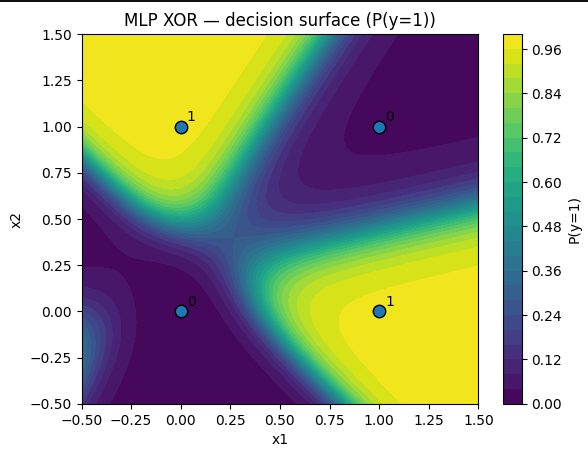
\includegraphics[width=0.24\textwidth]{img/balanced_set.png}
    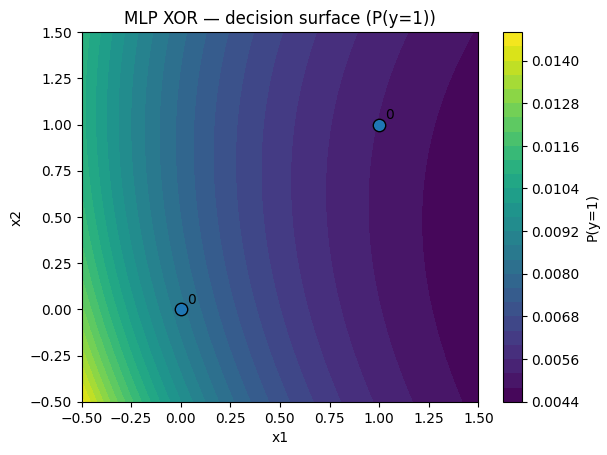
\includegraphics[width=0.24\textwidth]{img/unbalanced_set.png}
    \caption{Complete XOR (left) and the decision boundary with an incomplete training set.}
    
\end{figure}
\vspace{-6pt}

\vspace{-9pt}
\subsection*{Autoencoders to the rescue}
\vspace{-6pt}

An autoencoder \footnote{\url{https://github.com/artur-augustyniak/class_struggle/blob/2287420fa8b5882b3fc603b6660bb50810b764f1/notebooks/3_autoencoder_train_eval_inference.ipynb?short_path=827cbee\#L608}} is a neural network that learns to reconstruct its training input. 
The encoder compresses data into a hidden representation $z$, and the decoder tries to reconstruct the original input from it. 
The model is trained without labels by minimizing the reconstruction error \footnote{\url{https://github.com/artur-augustyniak/class_struggle/blob/2287420fa8b5882b3fc603b6660bb50810b764f1/notebooks/3_autoencoder_train_eval_inference.ipynb?short_path=827cbee\#L741}}.

Thus, it doesn’t need counterexamples; it doesn’t learn decisions but representations.

During inference \footnote{\url{https://github.com/artur-augustyniak/class_struggle/blob/2287420fa8b5882b3fc603b6660bb50810b764f1/notebooks/3_autoencoder_train_eval_inference.ipynb?short_path=827cbee\#L916}}, we pass new data through the network and measure the reconstruction error - 
a large value means that the sample is different from the training data.
The inner layer $z$ serves as an embedding - a compact representation of the data structure.

\vspace{-9pt}
\subsection*{Yet EDA - on limitations}
\vspace{-6pt}
Phishing domains are often created to resemble legitimate ones. 
Training on the entire corpus would result in an autoencoder that reconstructs legitimate domains.

I must restrain my ambitions. 
To do this, I perform EDA \footnote{\url{https://github.com/artur-augustyniak/class_struggle/blob/2287420fa8b5882b3fc603b6660bb50810b764f1/notebooks/1_eda.ipynb}} through clustering \footnote{\url{https://scikit-learn.org/stable/modules/generated/sklearn.cluster.HDBSCAN.html}}.

From the dataset, I select the cluster(s) of interest - in my case, domains with certain characteristics \footnote{\url{https://github.com/artur-augustyniak/class_struggle/blob/2287420fa8b5882b3fc603b6660bb50810b764f1/notebooks/2_eda_based_data_selection.ipynb}}.

\vspace{-9pt}
\subsection*{Preprocessing FTW}
\vspace{-6pt}
For the autoencoder to understand the data, it must be vectorized. 
Counting lengths, dashes, etc., loses semantic information, so I used TF-IDF statistics \footnote{\url{https://scikit-learn.org/stable/modules/generated/sklearn.feature_extraction.text.TfidfVectorizer.html}} on n-grams \footnote{\url{https://en.wikipedia.org/wiki/N-gram}}.

The TF-IDF vectorizer doesn’t preserve positional information or relationships between n-grams.
We can enforce minimal positional awareness by positional n-grams through adding start and end markers \footnote{\url{https://github.com/artur-augustyniak/class_struggle/blob/2287420fa8b5882b3fc603b6660bb50810b764f1/notebooks/3_autoencoder_train_eval_inference.ipynb?short_path=827cbee\#L498}}.


\vspace{-9pt}
\subsection*{Metrics and GOTO EDA}
\vspace{-6pt}

How to choose hyperparameters? I'm not a scientist, so I do it empirically. 
For network layer dimensions, remember that an autoencoder should compress the representation - a bottleneck is necessary \footnote{\url{https://github.com/artur-augustyniak/class_struggle/blob/2287420fa8b5882b3fc603b6660bb50810b764f1/notebooks/3_autoencoder_train_eval_inference.ipynb?short_path=827cbee\#L56}}.
Typically, if your validation loss increases while training loss decreases, you’ve trained too long or your model is too large \footnote{\url{https://github.com/artur-augustyniak/class_struggle/blob/2287420fa8b5882b3fc603b6660bb50810b764f1/notebooks/3_autoencoder_train_eval_inference.ipynb?short_path=827cbee\#L707}}.

A nice feature of the autoencoder is that we can apply PCA \footnote{\url{https://scikit-learn.org/stable/modules/generated/sklearn.decomposition.PCA.html}} to its embeddings 
and try to infer what the autoencoder has learned.\\You can find the repository with runnable code here:\\\url{https://github.com/artur-augustyniak/class_struggle/}.

\vspace{-9pt}
\begin{figure}[h!]
    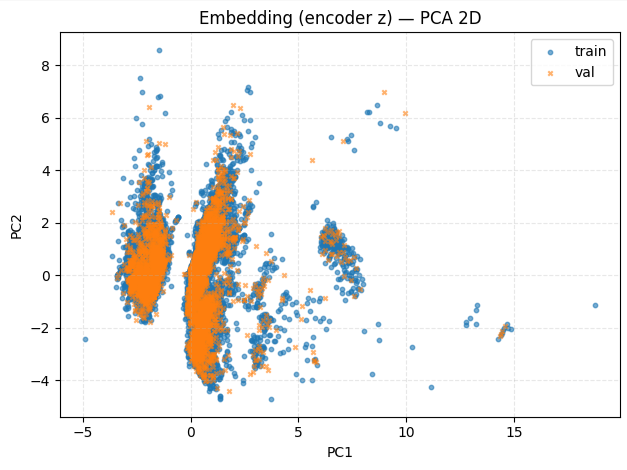
\includegraphics[width=0.24\textwidth]{img/small_ae.png}
    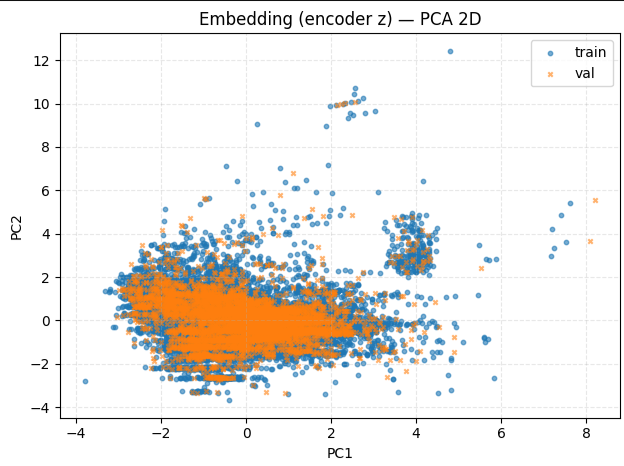
\includegraphics[width=0.24\textwidth]{img/big_ae.png}
    \caption{A small AE forced to learn classes (left) and a larger one capable of generalization. In each case, we are interested in the overlap between validation and training embeddings.}
\end{figure}
\vspace{-6pt}





\end{document}
